\documentclass{article}
\usepackage{fullpage,amsmath,url,cases}
\usepackage{natbib,longtable,graphicx,tikz}
\usepackage{subfig}
\usepackage{url}
%\@ifundefined{showcaptionsetup}{}{%
%\PassOptionsToPackage{caption=false}{subfig}}
\graphicspath{{./figures/}}
\usepackage{xcolor}
\usepackage{colortbl}
\definecolor{RubineRed}{RGB}{240, 0, 240}       % RubineRed  Approximate PANTONE RUBINE-RED
\usepackage{subfig}
\usepackage{listings}
\usepackage{color}

%%%%%%%%%%%%%%%%%%%%%%%%%%%%%%%%%% referencing %%%%%%%%%%%%%%%%%%%%%%%%%%%%%%%%%%
\usepackage{natbib}
\usepackage{hyperref}
\usepackage{xcolor}
\hypersetup{
    colorlinks,
    %linkcolor={red!50!black},
    linkcolor={black},
    citecolor={blue!50!black},
    urlcolor={blue!80!black}
}

%%%%%%%%%%%%%%%%%%%%%%%%%%%%%%%%%%%%%%%%%%%%%%%%%%%%%%%%%%%%%%%%%%%%%%%%%%%%%%%%
\usepackage[colorinlistoftodos]{todonotes}
%\usepackage[disable]{todonotes}

\newcounter{todocounter}
\newcommand{\todonum}[2][]
{\stepcounter{todocounter}\todo[#1]{\thetodocounter: #2}}

\newcommand{\done}[2][]
{\todo[color=green!40, #1]{#2}}

\newcommand{\donenum}[2][]
{\stepcounter{todocounter}\done[#1]{\thetodocounter: #2}}
%%%%%%%%%%%%%%%%%%%%%%%%%%%%%%%%%%%%%%%%%%%%%%%%%%%%%%%%%%%%%%%%%%%%%%%%%%%%%%%%

\definecolor{dkgreen}{rgb}{0,0.6,0}
\definecolor{gray}{rgb}{0.5,0.5,0.5}
\definecolor{mauve}{rgb}{0.58,0,0.82}

\lstset{frame=tb,
  language=Java,
  aboveskip=3mm,
  belowskip=3mm,
  showstringspaces=false,
  columns=flexible,
  basicstyle={\small\ttfamily},
  numbers=none,
  numberstyle=\tiny\color{gray},
  keywordstyle=\color{blue},
  commentstyle=\color{dkgreen},
  stringstyle=\color{mauve},
  breaklines=true,
  breakatwhitespace=true,
  tabsize=3
}
\lstset{language=bash}


\title{Supplementary Material}
\author{Sha Joe Zhu}
\date{}



\begin{document}
\maketitle{}
\listoftodos
\clearpage
\setcounter{page}{1}

\maketitle
\tableofcontents

\setcounter{section}{0}

\newpage
%\renewcommand{\thetable}{S\arabic{table}}
%\renewcommand{\thefigure}{S\arabic{figure}}


%%%%%%%%%% Merge with supplemental materials %%%%%%%%%%
%%%%%%%%%% Prefix a "S" to all equations, figures, tables and reset the counter %%%%%%%%%%
%\setcounter{section}{0}
\setcounter{equation}{0}
\setcounter{figure}{0}
\setcounter{table}{0}
\setcounter{page}{1}
\makeatletter
\renewcommand{\thesection}{Appendix~\arabic{section}}
\renewcommand{\theequation}{Appendix~\arabic{section}-equation~\arabic{equation}}
\renewcommand{\thefigure}{Appendix~\arabic{section}-figure~\arabic{figure}}
\renewcommand{\thetable}{Appendix\arabic{section}-table~\arabic{table}}
\renewcommand{\bibnumfmt}[1]{[Appendix~\arabic{section}#1]}
\renewcommand{\citenumfont}[1]{Appendix~\arabic{section}#1}
%%%%%%%%%% Prefix a "S" to all equations, figures, tables and reset the counter %%%%%%%%%%



%%%%%%% Start on new page
\renewcommand{\thepage}{Appendix\arabic{section}--\arabic{page}}

\section{Deconvoltion IBD methods}

%Overall we use mcmc methods.


%\todo{expand methods}

\subsection{Deconvolving mixed infection}
\subsubsection{Notations}
We use the same notations as \citet{Zhu2017} (see Table~\ref{tab:notation}). Our data, $D$, are the allele read counts of sample $j$ at a given site $i$, denoted as $r_{j,i}$ and $a_{j,i}$ for reference (REF) and alternative (ALT) alleles respectively.  These are assigned values of $0$ and $1$ respectively. Here we consider only bi-allelic loci, though future extension to include multi-allelic sites is simple.  The empirical allele frequencies within a sample (WSAF) $p_{j,i}$ and at population level (PLAF) $f_i$ are calculated by $ \frac{a_{j,i}}{a_{j,i} + r_{j,i}}$ and $ \frac{\sum_j a_{j,i}}{\sum_j a_{j,i} + \sum_j r_{j,i}}$ respectively. Since all data in this section refers to the same sample, we drop the subscript $j$ from now on.

\begin{table}[htb]\centering
\begin{tabular}{c|c}\hline
$i$              & Marker index\\
$j$              & Sample index \\
$r$              & Read count for reference allele \\
$a$              & Read count for alternative allele \\
$f$              & Population level allele frequency (PLAF) \\
$n$              & Number of strains within sample \\
$l$              & Sequence length \\
$\mathbf{w}$      & Proportions of strains \\
%$\mathbf{x}$	& Log titre of strains \\
$\mathbf{h}_{i}$ & Allelic states of $n$ parasite strains at site $i$ \\
$h_{k,i}$   & Allelic state of parasite strain $k$ at site $i$\\
$p$              & Observed within sample allele frequency (WSAF) \\
$q$              & Unadjusted expected WSAF  \\
$\pi$            & Adjusted expected WSAF \\
%$\Xi$            & Reference panel\\
%$\xi_{k,i}$     & Allelic state of reference panel strain $k$ at site $i$\\
%$G$              & Scaling factor used for genetic map\\
$e$              & Probability of read error\\
$\mathcal{S}$ & IBD state \\
$\mathcal{H}$ & haplotype state \\
\hline
\end{tabular}
\caption{Table summarising the notation used in this article.}\label{tab:notation}
\end{table}

\subsubsection{Model}

We describe the mixed infection problem by considering the number of strains, $n$, the relative abundance of each strain, $\mathbf{w}$, and their allelic states, $\mathbf{h}_{i}$. In addition to \citet{Zhu2017}, we also infer the IBD-state $\mathcal{S}_{i}$, which describes the strain relationships at each site $i$. For example, for three strains, the IBD-state could be one of the five cases: (1) all strains are IBD; (2) all strains are not IBD; (3)(4)(5) only two strains are IBD. To simplify our problem, we assume independence between each marker, and drop the subscript $i$ from now on. Similar to \citet{Jack2016}, we use a Bayesian approach and define the posterior probabilities of $n$, $\mathbf{w}$, $\mathbf{h}$ and $\mathcal{S}$,  as:

\begin{equation}
P(n, \mathbf{w}, \mathbf{h}, \mathcal{S}| e, D) \propto L(n, \mathbf{w}, \mathbf{h}, \mathcal{S} | e, D) \times P(n, \mathbf{w}, \mathbf{h}, \mathcal{S}), \label{eqn:post}
\end{equation}
where $e$ is the read error rate.

\noindent We assume a prior in which the haplotypes of the $n$ strains are independent of each other and dependent only on the IBD state. Let $\mathcal{H}$ be the haplotype state that is derived from the IBD state $\mathcal{S}$. We assume uniform prior on $\mathcal{H}|\mathcal{S}$. For example, if $n=3$ and only strains 1 and 2 are IBD, the haplotype states $\mathcal{H}$ could be $\{0,0,0\}$; $\{0,0,1\}$; $\{1,1,0\}$ and $\{1,1,1\}$. Therefore, we can decompose the joint prior as:
\begin{equation}
P(n, \mathbf{w}, \mathbf{h}, \mathcal{S}) = P(n) \times P(\mathbf{w}|n) \times P(\mathbf{h} , \mathcal{S}|n),
\end{equation}
where
\begin{equation}
P(\mathbf{h}, \mathcal{S}|n) = P(\mathcal{S}|n) \times \sum_{\xi \in \mathcal{H}} P(\mathbf{h} | \xi) \times P(\xi|\mathcal{S}).
\label{eqn:}
\end{equation}


\noindent For details of the likelihood and the prior on the proportions see \citet{Zhu2017} sections 2.2.1 and 2.2.2. We use the following expression for the expected WSAF $q$, as:
\begin{equation}
q = \mathbf{w}\cdot\mathbf{h}.\label{eqn:qij_full_sum}
\end{equation}

        %ll1<- lbeta(e1*c+alt.cts[site], (1-e1)*c+(read.depths[site]-alt.cts[site]));
        %ll2<- -lbeta(e1*c, (1-e1)*c);
        %ll<-ll1+ll2;
        %ln<- exp(ll-max(ll));
        %ln<-ln/sum(ln);
        %mn<-sum(ln*p.grid); # Compute the posterior, then normalize by the mean?
        %vr<-sum(ln*p.grid^2)-mn^2;
        %llk.apx[site,]<-(mn*(1-mn)/vr-1)*c(mn, 1-mn);


\noindent The data, which can be summarised by the reference and alternative allele read counts at each site, is modelled through a beta-binomial distribution given the expected WSAF.  We model the data at distinct segregating sites as independent.  Thus the likelihood function  in Eqn.~\eqref{eqn:post} is only dependent on the haplotypes present and their frequencies through their contribution to $q_{i}$.

%; i.e. $L(n, \mathbf{w}, \mathbf{h}, | \Xi, e, D) = \prod_{i=1}^l L(q_i | \Xi, e, D)$.

To incorporate sequencing error, we modify the expected WSAF such that the allele frequency of `REF' read as `ALT' is $(1 - q_i)e$, and the allele frequency of `ALT' read as `REF' is $q_ie$. Thus, the adjusted expected WSAF becomes:

\begin{equation}
\pi_i = q_i + (1 - q_i)e - q_ie = q_i + (1 - 2q_i)e.\label{eqn:adj_q}
\end{equation}

\noindent We model over-dispersion in read counts relative to the Binomial using a Beta-binomial distribution. Specifically, the read counts of `ALT' are identically and independently distributed (i.i.d.) Bernoulli random variables with probability of success $v_i$; i.e. $a_i \sim Binom(a_i + r_i, v_i)$, and $v_i \sim Beta(\alpha, \beta)$, where $E(v_i) = \alpha/(\alpha+\beta) = \pi_{i}$. This is achieved by setting $\alpha = c\cdot \pi_{i} $ and $\beta = c\cdot (1-\pi_{i})$, such that the variance of the WSAF is inversley proportion to $c$.  Combined, we have:

\begin{equation}
L(q_{i}| e, D) \propto \frac{\Gamma(a_i + c\cdot \pi_{i}) \Gamma(r_i + c\cdot (1-\pi_{i}))}{\Gamma(c\cdot \pi_{i})\Gamma(c\cdot (1-\pi_{i}))}. \label{eqn:llk}
\end{equation}


%\subsubsection{Metropolis-Hastings update for proportions}\label{sec:updateP}
%\todo{To keep this? or just mention this is the same as \citet{Zhu2017}}
%We update $\mathbf{w}|n$, through the underlying log titres, $\mathbf{x}|n$. Specifically, we choose $i$ uniformly from $n$ and propose new $x_i'$s from $x_i' = x_i + \delta x$, where $\delta x \sim N(0, \sigma^2/s)$, and $s$ is a scaling factor. The new proposed proportion is therefore $\frac{\exp(x_k')}{\sum_{k=1}^n \exp(x_k')}$. Since the proposal distribution is symmetrical, the Hastings ratio is 1. A new update is accepted with probability

 %$$\min\left(1, \frac{P(\mathbf{w}'|n)}{P(\mathbf{w}|n)} \frac{L(\mathbf{w}', \mathbf{h}, {\mathcal S} | e, D)}{L(\mathbf{w}, \mathbf{h}, {\mathcal S} | e, D)}\right).$$

%\subsubsection{Gibbs sampling for haplotype and IBD-configuration update}


%\paragraph{Prior on $\mathcal{S}|n$}

%Inbreeding coefficient.


%To perform inference about the haplotypes present and their proportions we use Markov chain Monte Carlo (MCMC). We use a Metropolis-Hastings algorithm to sample proportions ($\mathbf w$) given $\mathbf h$; and use a Gibbs sampler to update $\mathbf h$ for a given $\mathbf w$, with two types of update: a single haplotype and a pair of haplotypes.

%\begin{itemize}
  %\item Likelihood
  %\item MCMC
%\end{itemize}

%Hidden markov model, $\mathcal{S}_{i}$ transition probability $t_{i, i+1}$, and emission probability $P(\mathbf{h} | \xi)$.



\subsection{Implementation details}
\begin{itemize}
%We then compute the likelihood as $\frac{x^{\alpha-1}(1-x)^{\beta-1}} {\Beta(\alpha,\beta)}\!$, where

%${\displaystyle \mathrm {B} (\alpha ,\beta )={\frac {\Gamma (\alpha )\Gamma (\beta )}{\Gamma (\alpha +\beta )}}}$

  \item {\bf Likelihood surface} We consider compute the likelihood of a given WSAF as \cite{Zhu2017} Equation~(5), and make the likelihood surface for WSAF. Given the integrated likelihood surface, we compute the likelihood for WSAF = 0 and WSAF = 1. We use these two values as shape parameters of a beta distribution, $\alpha = llk_{0}$ and $\beta = llk_{1}$, instead of computing the likelihood of a given WASF, we integrate the likelihood over the possible span of WSAF.

%ibd state configuration, haplotype state configuration.

\item {\bf MCMC parameters for deconvolution}

\begin{itemize}
\item {\bf Number of strains}. As described above, we aim to infer more strains than are actually present, starting the MCMC chain with a fixed $n$, which has a default of $5$. At the point of reporting, we discard strains with a proportion less than a fixed threshold, typically $0.01$.

\item {\bf Parameters}. \textcolor{black}{The parameter $c$ (Equation~\eqref{eqn:llk}) reflects how much data are available. The mean coverage of the validation data set ranges from 106.20 to 147.04, with a mean of 124.487.} In practice, we set the parameters $c=100$; $\eta = 0$, \textcolor{black}{$\sigma^2 = 5$ which are adjusted accordingly when working with extremely unbalanced samples (Section \ref{sec:prior} and supplementary material)}.  We set the read error rate as 0.01 and the rate of mis-copying as 0.01.

\item {\bf Recombination rate and scaling}. We assume a uniform recombination map, where the genetic distance between loci $i$ and $i+1$ is computed by $\psi_i = D_i / d_m$ where $D_i$ denotes the physical distance between loci $i$ and $i+1$ in nucleotides and $d_m$ denotes the average recombination rate in Morgans bp$^{-1}$. We use the recombination rate for {\it P. falciparum} of 15,000 base pairs per centiMorgan as reported by \citet{Miles2016}. The recombination rate is scaled by a factor $G$, which reflects the effective population size, rate of inbreeding and size and relatedness of the reference panel. \textcolor{black}{In practice, we deconvolve over 1 million markers in field samples. We use a value of $G=20$ to ensure small values for recombination probabilities between any two markers, with a mean of 0.015. A large value of $G$ relaxes the reference panel constraint, becoming an LD free model when $G$ is infinity.  In practice, inference seems largely insensitive to choices around this parameter.}  The scaled genetic distance $G\psi$ is used to compute the transition probability of switching from copying reference haplotype $a$ to reference haplotype $b$ (see Supplementary Materials for details).

\item {\bf Update without linkage disequilibrium}. For initialising the chain, or if the markers present are very widely spaced, linkage disequilibrium can be ignored, which is equivalent to setting the genetic distance between adjacent loci to be infinitely high.  Under these circumstances, the haplotype updates become much simpler and depend only on the population-level allele frequency (PLAF), for example as estimated from the reference panel or provided independently.

\item {\bf Reporting} We aim to provide users with a single point estimate of the haplotypes and their proportions, although the full chain is also available for analysis.  To achieve this we report values at the last iteration - i.e. we report a single sample from the posterior.  However, to measure robustness, we typically repeat the deconvolution with multiple random starting points\textcolor{black}{. We use a majority vote rule on the inferred number of strains; we then select the chain with the lowest average deviance (after removing the burn-in) as our estimate. The deviance measures the difference in log likelihood between the fitted and saturated models, the latter being inferred by setting the WSAF to that of the observed values.} These parameters can be modified by users to achieve a preferred balance between computational speed and confidence.  By default, we set the MCMC sampling rate as 5, with the first 50\% of samples removed as burn in and 800 samples used for estimation.

\item {\bf Reference panel construction}. To infer clonal samples for the reference panel we use the Pf3k project data, running the algorithm without LD on all samples and identifying those with a dominant haplotype (proportion > 0.99) as clonal.  These clonal samples are grouped by region of sampling to form location-specific reference panels.  In addition, we have included a number of reference strains, described in more detail below.

\end{itemize}

  %\item {\bf Extract crossover events} We treat genome regions of which IBD posterior probabilities greater than 90\% as IBD blocks. Regions that are not identified by a particular IBD region are crossover event candidates. We identify the candidate region of which two sides belong to different IBD blocks as a crossover event.

%\item {\bf MCMC parameters for recombination map and smoothing}
%We burn the first 10\% of the MCMC chain, and draw every 5th sample of the chain. To collect 1000 samples for each SNP interval.
\end{itemize}


\subsection{Data filtering}
We find markers with high frequencies in both reference and alternative allele count can mislead our model to fit extra strains. We then use a threshold of ≥ 99.5\% coverage (default) to identify markers with extremely high allele counts. These markers often appears in clusters as a result of poor mapping. We further expand this list of potential “bad markers” by considering their nearest 10 neighbours on both sides along the genome, and identify the nearest markers as “to be excluded” if overlaps are found (see Figure S2.1).

\begin{figure}[htp]
  \centering{}
  \subfloat[][]{
    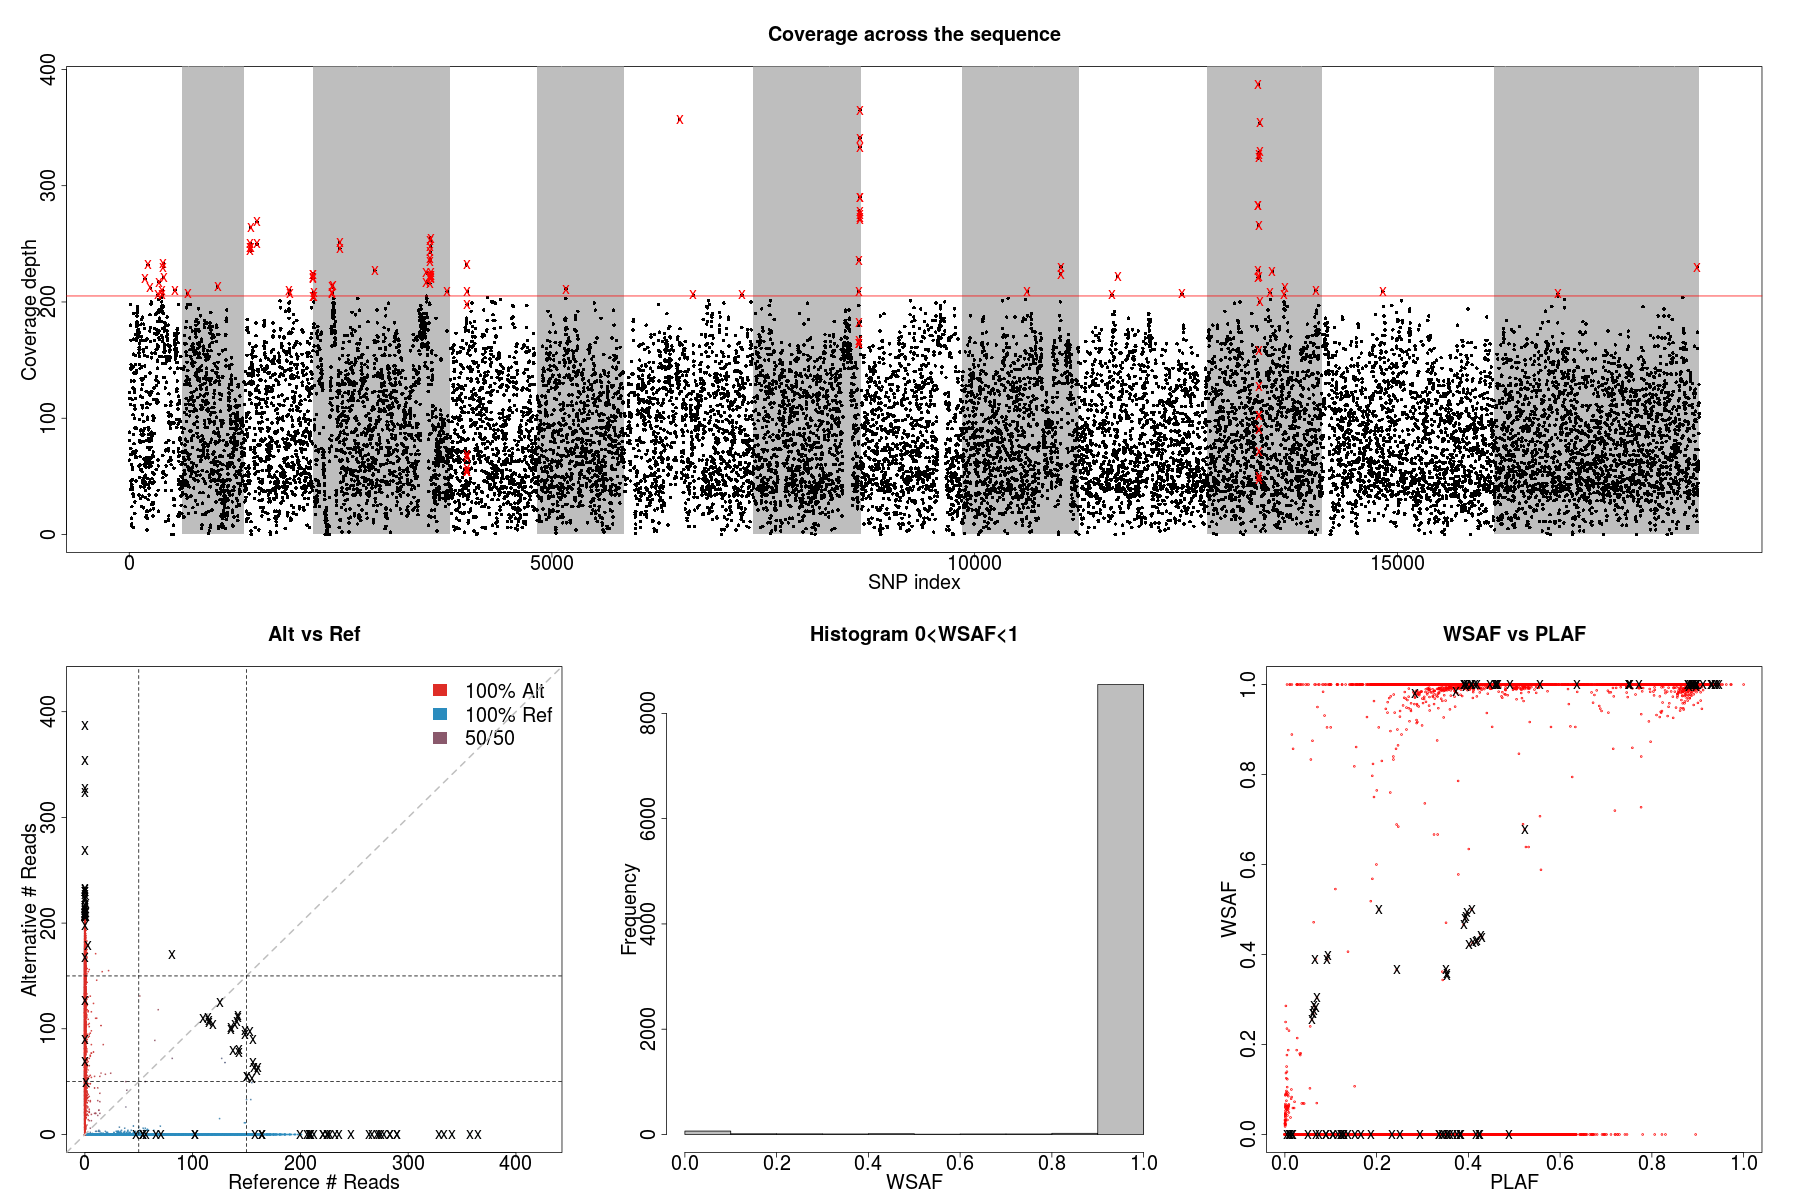
\includegraphics[width=0.7\textwidth]{PG0415-CaltVsRefAndWSAFvsPLAF.png}
  }\\
  \subfloat[][]{
  \includegraphics[width = 0.45\textwidth]{{PG0415-CNopanel.ring}.png}
  }
  \subfloat[][]{
    \includegraphics[width=0.45\textwidth]{{PG0415-CNopanel.filtered.ring}.png}
  }\\
  %\subfloat[][]{
    %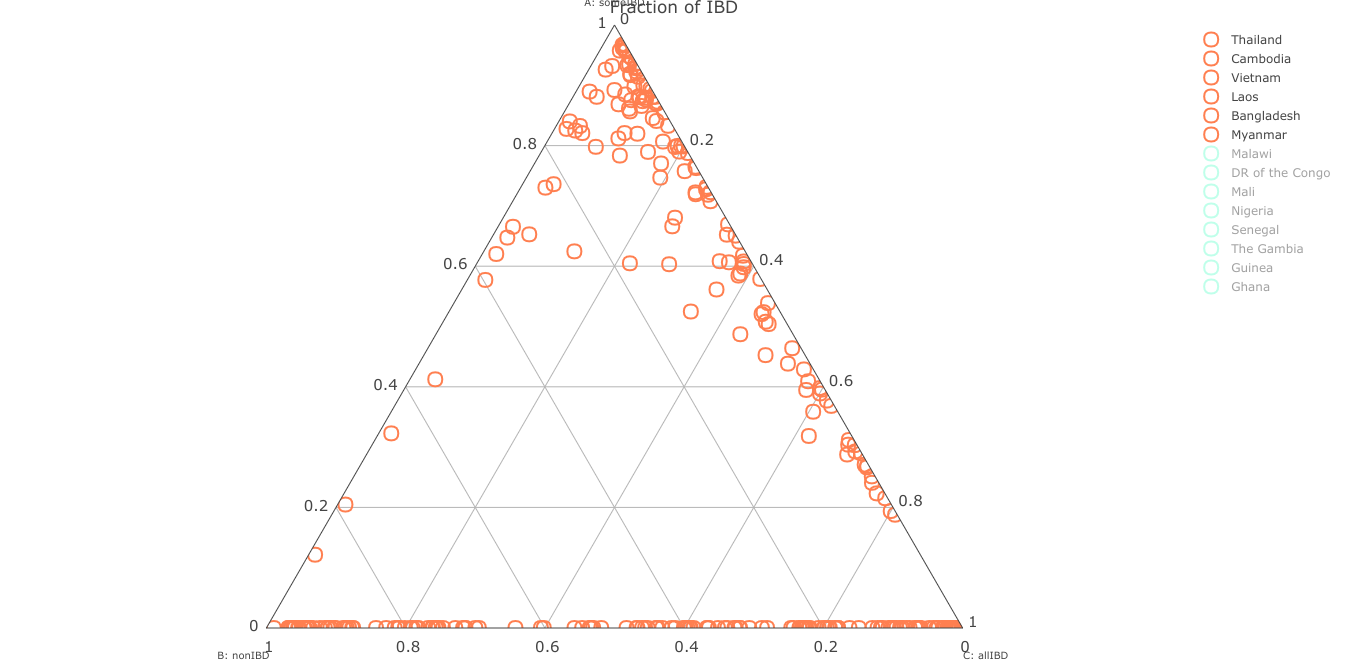
\includegraphics[width=0.8\textwidth]{ibdDistribution_asia.png}
  %}\\
  \caption{We observe a small number of heterozygous sites with high coverage (marked as crosses above), which can potentially mislead our model to over-fit the data with additional strains.
  }
  \label{fig:fitering}
\end{figure}


\subsection{Commands}

\linespread{1}
\begin{lstlisting}
vcf="PD0165-C.vcf.gz"
plaf="plaf.1"
panel="clonalSamples.1.mostDiverse15.txt"
exclude="exclude.1"

common="-vcf ${vcf} -plaf ${plaf} -exclude ${exclude}"
mcmcCommon=" -panel ${panel} -k 2 -nSample 250 -rate 8 -burn 0.67 -seed 1"

prefix="PD0165-C-noIBD"
dEploid ${common} ${mcmcCommon} -o ${prefix}
~/DEploid/utilities/interpretDEploid.r ${common} -dEprefix ${prefix} -o ${prefix}

prefix="PD0165-C"
dEploid ${common} ${mcmcCommon} -o ${prefix} -ibd
~/DEploid/utilities/interpretDEploid.r ${common} -dEprefix ${prefix} -o ${prefix} -ibd

~/pfPvRecombMap/plotIBD.r ${prefix} ${plaf} ${vcf}
\end{lstlisting}


\subsection{Bench mark}

Our deconvolution experiment used 17,530 sites for all experiments in the rest of this section, unless specified otherwise.

To evaluate accuracy of estimates we used the effective number of strains, calculated as  1/∑w2i1/∑wi2 , which reflects the number and proportions of strains present. We also assessed sensitivity of estimates to the number of fitted strains (3 or 5). Typically, we find consistent inference of the effective number of strains regardless of the assumption of number of strains or the use of LD information (see Fig. 1). The deviance between the expected and inferred proportions per sample is bounded by the inverse of the deviation between expected and observed effective number of strains


Against DEploid without using IBD methods.
\begin{figure}[htp]
  \centering{}
  \subfloat[][]{
  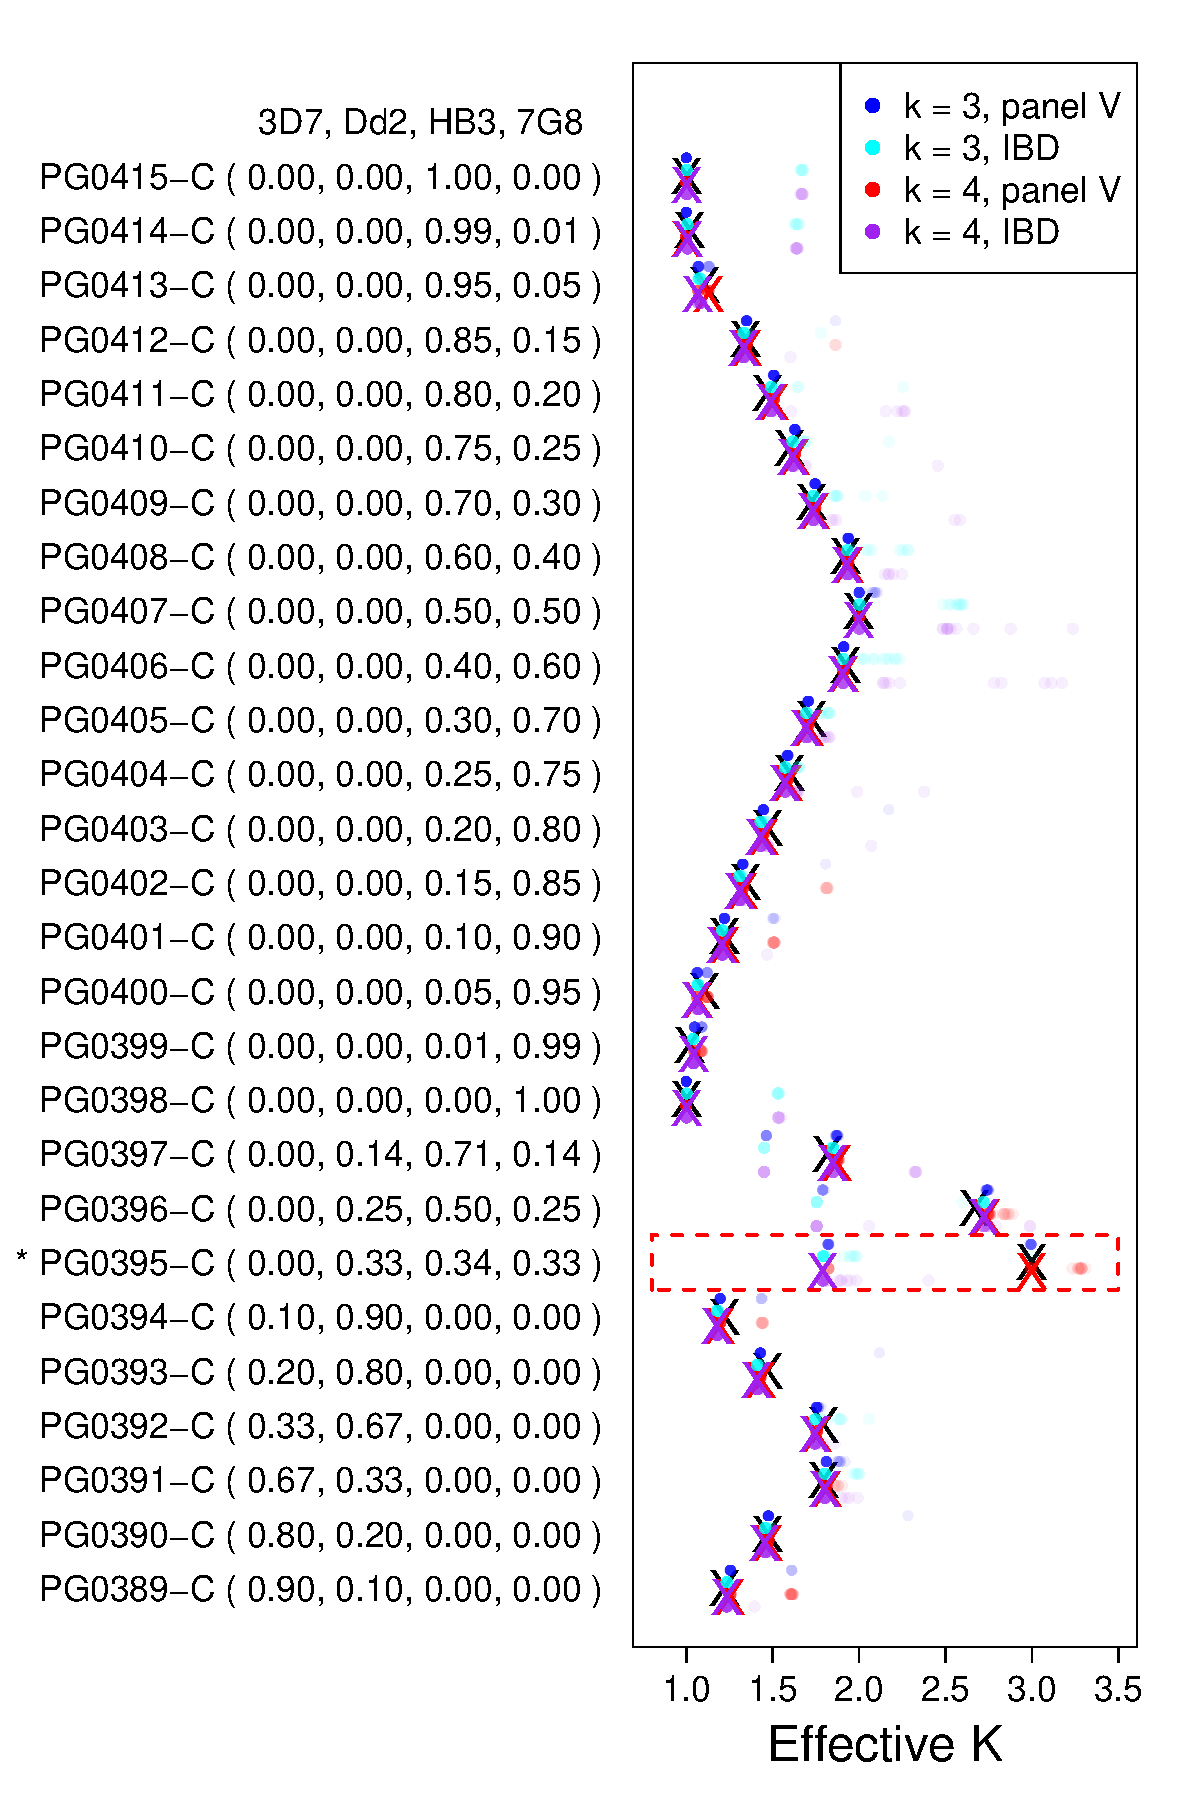
\includegraphics[width = 0.65\textwidth]{eff_k_both.pdf}
  }
  \caption{Simulation results}
\end{figure}
\begin{figure}
  \ContinuedFloat
  \centering
  \subfloat[][]{
  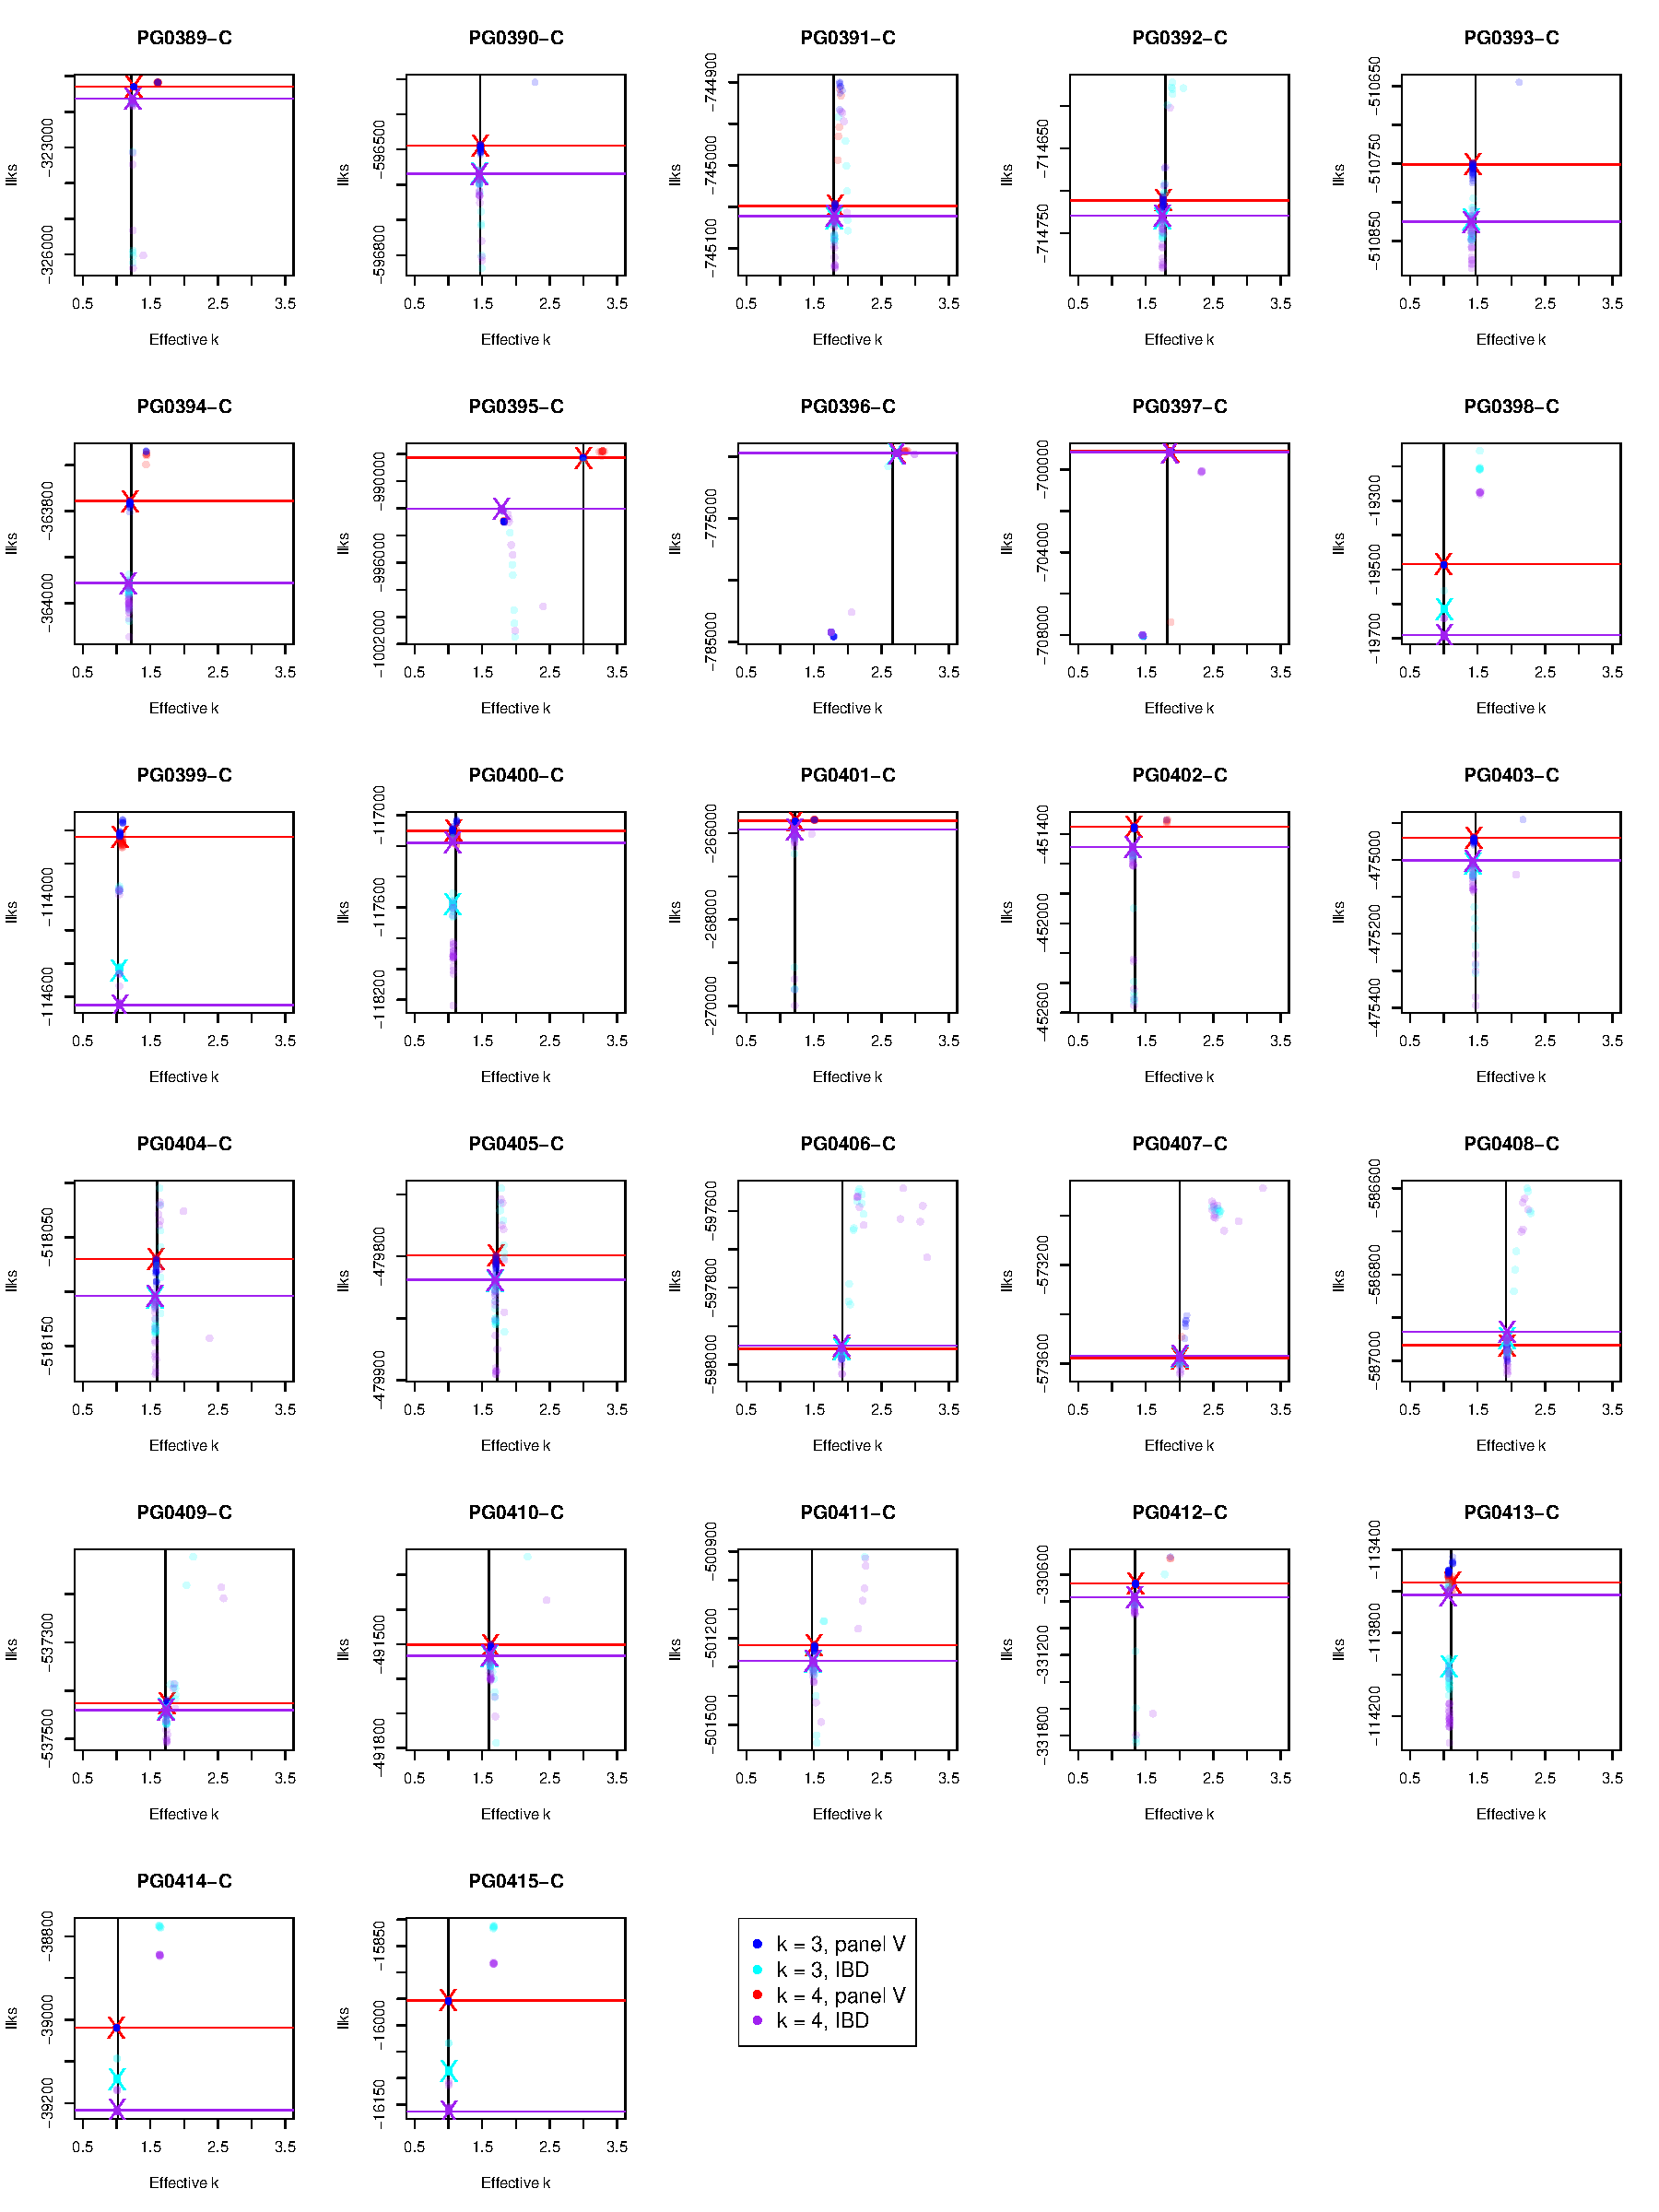
\includegraphics[width = 0.85\textwidth]{eff_k_vs_llk.pdf}
  }
  \caption{Simulation results}
\end{figure}

\begin{figure}
  \ContinuedFloat
  \centering
  \subfloat[][]{
  \includegraphics[width = 0.8\textwidth]{DEploid_IBD_haps_compare.pdf}
  }
  \caption{Simulation results}
\end{figure}


\subsection{Identifier problem}
Since we use panel free, for equal proportions it is difficult to identify.
Without a reference panel, we assume independence between loci, it is difficult to identify cases between $\{\frac{1}{3},\frac{1}{3},\frac{1}{3}\}$ and $\{\frac{1}{3},\frac{2}{3}\}$, or
$\{\frac{1}{4},\frac{1}{4}, \frac{1}{4}, \frac{1}{4}\}$ and $\{\frac{1}{4},\frac{1}{4}, \frac{1}{2}\}$, or $\{\frac{1}{5},\frac{1}{5}, \frac{1}{5}, \frac{1}{5}, \frac{1}{5}\}$ and $\{\frac{1}{5},\frac{1}{5}, \frac{3}{5}\}$, $\{\frac{1}{5},\frac{2}{5}, \frac{2}{5}\}$ and
$\{\frac{1}{5},\frac{1}{5}, \frac{1}{5}, \frac{2}{5}\}$.
%\subsection{Simulation study}


%To estimate COI, relative proportions and strain haplotypes we use DEploid [Zhu et al., 2017] on high quality biallelic SNP data (both coding and non-coding variants tagged with PASS at the QUAL column in the VCF file). In order to improve the accuracy of the deconvolution process and improve efficiency, we first split the Pf3k data into groups, based on genetic similarity. We compute genetic distances between two samples following

%where l represents an arbitrary locus, L denotes the total number of loci, and  indicates the non-reference within-sample allele frequency for sample s at locus l.  is then given by

%where  is the number of read counts supporting the alternative allele in sample s at locus l, and  is the number of read counts supporting the reference allele in sample s at locus l.
%We find that samples from the same geographical region differentiate into clear clusters. We use this initial grouping as the base for defining the reference panels that assist the deconvolution procedure. Our definition of geographical groups is
%Africa
%Malawi, Congo.
%Ghana (Kassena).
%Nigeria, Senegal, Mali.
%The Gambia, Guinea, Ghana (Kintampo).
%Asia
%Cambodia (Pursat), Cambodia (Pailin), Thailand (Sisakhet).
%Vietnam, Laos, Cambodia (Ratanakiri), Cambodia (Preah Vihear).
%Bangladesh, Myanmar, Thailand (Mae Sot), Thailand (Ranong).

%\newpage
%%\renewcommand{\thetable}{S\arabic{table}}
%\renewcommand{\thefigure}{S\arabic{figure}}


%%%%%%%%%% Merge with supplemental materials %%%%%%%%%%
%%%%%%%%%% Prefix a "S" to all equations, figures, tables and reset the counter %%%%%%%%%%
%\setcounter{section}{0}
\setcounter{equation}{0}
\setcounter{figure}{0}
\setcounter{table}{0}
\setcounter{page}{1}
\makeatletter
\renewcommand{\thesection}{Appendix~\arabic{section}}
\renewcommand{\theequation}{Appendix~\arabic{section}-equation~\arabic{equation}}
\renewcommand{\thefigure}{Appendix~\arabic{section}-figure~\arabic{figure}}
\renewcommand{\thetable}{Appendix\arabic{section}-table~\arabic{table}}
\renewcommand{\bibnumfmt}[1]{[Appendix~\arabic{section}#1]}
\renewcommand{\citenumfont}[1]{Appendix~\arabic{section}#1}
%%%%%%%%%% Prefix a "S" to all equations, figures, tables and reset the counter %%%%%%%%%%



%%%%%%% Start on new page
\renewcommand{\thepage}{Appendix\arabic{section}--\arabic{page}}


%\section{Deconvolution example with sample PD0577-C}

%The following example shows a specific {\textmd DEploid} command to deconvolute the mixed sample {\textmd PD0577-C}:
%\linespread{1}
%\begin{lstlisting}
%dEploid -ref PD0577-C_ref.txt \
    %-alt PD0577-C_alt.txt \
    %-plaf asia-1_PLAF.txt \
    %-exclude asia-1_exclude.txt \
    %-panel asia-1_panel.txt \
    %-o PD0577-C.deconv \
    %-seed 5 \
    %-nSample 250 \
    %-rate 8 \
    %-burn 0.67 \
    %-k 3 \
    %-exportPostProb
%\end{lstlisting}
%\linespread{1.5}
%where ``{\tt -ref PD0577-C\_ref.txt}'' and ``{\tt -alt PD0577-C\_alt.txt}'' define the input text files \footnote{The Pf3k data was deconvoluted using DEploid version v0.1-beta. Recent versions can take VCF files as input as well.} that record the reference and alternative read counts respectively; ``{\tt -plaf asia-1\_PLAF.txt}'' contains the population allele frequencies calculated from total read counts. Note that we use option ``{\tt -exclude asia-1\_exclude.txt}'' to skip deconvoluting monomophic sites; ``{\tt -panel asia-1\_panel.txt}'' specifies a text file including haplotypes of samples listed in Table~\ref{tab:panelSamples}; options ``{\tt -nSample}'', ``{\tt -rate}'' and ``{\tt -burn}'' specify the total number of MCMC samples to take, the sampling rate and the burning rate of the MCMC chain respectively. For detailed documentation, please see \url{http://deploid.readthedocs.io/en/latest/input.html}.

%\linespread{1}
%\begin{lstlisting}
%dEploid -ref PD0577-C_ref.txt \
    %-alt PD0577-C_alt.txt \
    %-plaf asia-1_PLAF.txt \
    %-exclude asia-1_exclude.txt \
    %-panel asia-1_panel.txt \
    %-o PD0577-C.deconv \
    %-painting PD0577-C.deconv.hap
%\end{lstlisting}
%\linespread{1.5}



%We use a utility {\tt R} script to plot and interpret the output produced by DEploid. The following command is used to generate Figures~\ref{fig:PD0577} (a) -- (e).
%\linespread{1}
%\begin{lstlisting}
%R --slave "--args
    %-ref PD0577-C_ref.txt
    %-alt PD0577-C_alt.txt
    %-plaf asia-1_PLAF.txt
    %-exclude asia-1_exclude.txt
    %-o PD0577-C.deconv
    %-dEprefix PD0577-C.deconv" < ~/DEploid/utilities/interpretDEploid.r
%\end{lstlisting}
%\linespread{1.5}
%where flags ``{\tt -ref}'', ``{\tt -alt}'', ``{\tt -plaf}'' and ``{\tt -exclude}'' are used in the same manner as in the previous example.


%\begin{figure}[ht]
%\centering
%\caption{Sample {\textmd PD0577-C} deconvolution with Reference Panel Asia-1. (a) Diagnostic panels from the \texttt{DEploid} output. The top three panels are used as data exploration of sample {\textmd PD0577-C}. From left to right, it shows: 1. Alternative read counts vs reference read counts. 2. Histogram of the allele frequencies within sample.
%3. Allele frequencies at the population level (PLAF) vs allele frequencies within the sample (WSAF): red dots show observed WSAF, which is calculated by read counts; blue does show the expected WSAF. The next three plots from left to right show: 1. MCMC samples for the strain proportions, with the fraction of each color indicating the proportion of a different strain at each MCMC sample. The three colored blocks suggest that there are three strains within sample {\textmd PD0577-C}, with proportions approximately 1/4, 1/4 and 1/2.
%2. Expected WSAF vs observed WSAF. We use the correlation between the observed and expected WSAF as a sanity check for our model. A low correlation suggests poor fitting.
%3. Log likelihood of the MCMC chain. This figure is used to indicate whether the MCMC has converged. The colored dots mark the likelihoods of the model when specific MCMC steps are used: updating the strain porportions, painting a single haplotype and painting a pair of haplotypes are marked in green red and blue respectively. (b) Expected WSAF (blue) and observed WSAF (red) across the genome. This figure highlights the genome diversity within the mixed sample across the genome. (c) (d) and (e) show the posterior painting probabilities for the deconvoluted strains when using the Reference Panel Asia-1. Each panel represents the posterior probability of a chromosome. Chromosomes 1 -- 14 are ordered from left to right, then top to bottom.
%}\label{fig:PD0577}
%\end{figure}




%\newpage
%%\renewcommand{\thetable}{S\arabic{table}}
%\renewcommand{\thefigure}{S\arabic{figure}}


%%%%%%%%%% Merge with supplemental materials %%%%%%%%%%
%%%%%%%%%% Prefix a "S" to all equations, figures, tables and reset the counter %%%%%%%%%%
%\setcounter{section}{0}
\setcounter{equation}{0}
\setcounter{figure}{0}
\setcounter{table}{0}
\setcounter{page}{1}
\makeatletter
\renewcommand{\thesection}{Appendix~\arabic{section}}
\renewcommand{\theequation}{Appendix~\arabic{section}-equation~\arabic{equation}}
\renewcommand{\thefigure}{Appendix~\arabic{section}-figure~\arabic{figure}}
\renewcommand{\thetable}{Appendix\arabic{section}-table~\arabic{table}}
\renewcommand{\bibnumfmt}[1]{[Appendix~\arabic{section}#1]}
\renewcommand{\citenumfont}[1]{Appendix~\arabic{section}#1}
%%%%%%%%%% Prefix a "S" to all equations, figures, tables and reset the counter %%%%%%%%%%



%%%%%%% Start on new page
\renewcommand{\thepage}{Appendix\arabic{section}--\arabic{page}}


%\section{Genome fractions of IBD regions}

%%\subsection{\textcolor{red}{Filtering samples by coverage}}

%\begin{figure}[h]
%\centering
%\missingfigure[figwidth=\textwidth]{genome IBD fractions? }
%\caption{}
%\end{figure}



\begin{figure}[htp]
  \centering{}
  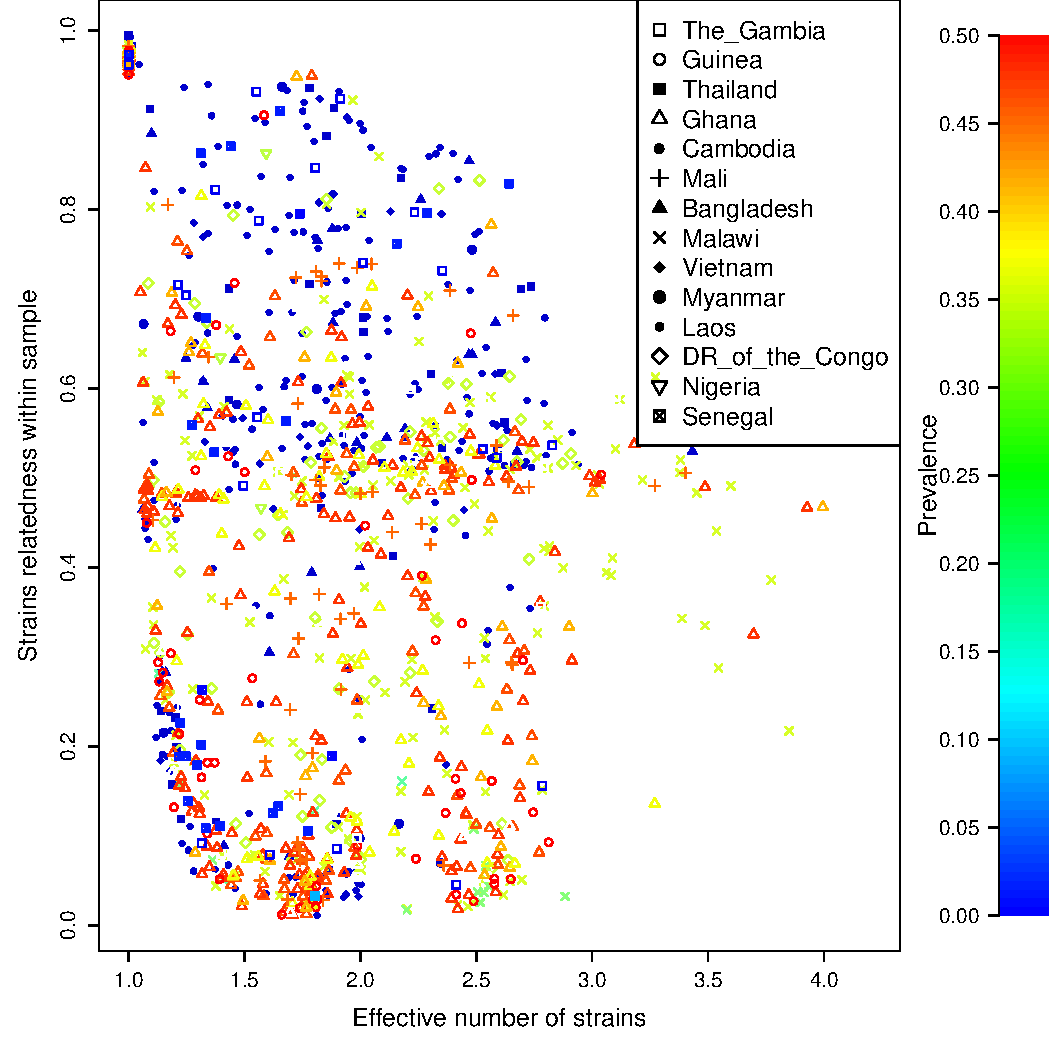
\includegraphics[width=0.8\textwidth]{effK_IBD_colored.pdf}
  \caption{}\label{fig:tmp1}
\end{figure}



\begin{figure}[htp]
  \centering{}
  \includegraphics[width=0.8\textwidth]{{llkDiff_vs_eff_k_diff.ibd}.png}
  \\
  \includegraphics[width=0.8\textwidth]{{llkDiff_vs_eff_k_diff}.png}
  \caption{}\label{fig:tmp2}
\end{figure}


\section{IBD state posterior probabilities of all population}
\subsection{Monitoring malaria epidemic from the IBD posterior probability}



\begin{thebibliography}{}

\bibitem[\protect\citeauthoryear{Browning and Browning}{Browning and
  Browning}{2007}]{Browning2007}
Browning, S.~R. and B.~L. Browning (2007)
\newblock Rapid and accurate haplotype phasing and missing-data inference for
  whole-genome association studies by use of localised haplotype clustering.
\newblock {\em Am. J. Hum. Genet.\/}~{\em 81\/}(5), 1084--1097.

\bibitem[\protect\citeauthoryear{Neafsey}{Neafsey}{2012}]{Neafsey2012}
Neafsey, D. {\em et al}.(2012)
\newblock The malaria parasite {\it Plasmodium vivax} exhibits greater genetic diversity than {\it Plasmodium falciparum}.
\newblock {\em Nature Genetics\/}~{\em 44\/}(9), 1046--1052.

\bibitem[\protect\citeauthoryear{Wegmann}{Wegmann}{2011}]{Wegmann2011}
Wegmann, D. {\em et al}.(2011)
\newblock Recombination rates in admixed individuals identified by ancestry-based inference.
\newblock {\em Nature Genetics\/}~{\em 43\/}, 847--894.

\bibitem[\protect\citeauthoryear{Hinch}{Hinch}{2011}]{Hinch2011}
Hinch, A.G. {\em et al}. (2011))
\newblock The landscape of recombination in African Americans.
\newblock {\em Nature\/}~{\em 476}, 170--175.

\bibitem[\protect\citeauthoryear{Henden}{Henden}{2016}]{Henden2016}
Henden, L. {\em et al}. (2016))
\newblock Detecting selection signals in {\it Plasmodium falciparum} using identity-by-descent analysis,
\newblock {\em bioRxiv.\/}, 088039.


\bibitem[\protect\citeauthoryear{Mu}{Mu}{2005}]{Mu2005}
Mu, J. {\em et al}. (2005)
\newblock Recombination Hotspots and Population Structure in {\it Plasmodium falciparum}.
\newblock {\em PLOS Biology.\/}~{\em 3}, e335.


\bibitem[\protect\citeauthoryear{Lopez}{Lopez}{2012}]{Lopez2012}
Lopez A. {\em et al}. (2012)
\newblock Genetic diversity of {\it Plasmodium vivax} and {\it Plasmodium falciparum} in Honduras.
\newblock {\em Malaria Journal.\/}~{\em 11}, 391.

\bibitem[\protect\citeauthoryear{Jiang}{Jiang}{2011}]{Jiang2011}
Jiang, H. {\em et al}. (2011)
\newblock High recombination rates and hotspots in a {\it Plasmodium falciparum} genetic cross.
\newblock {\em Genome Biology.\/}~{\em 12}, R33.


\bibitem[\protect\citeauthoryear{Miles, Iqbal, Vauterin, Pearson, Campino,
  Theron, Gould, Mead, Drury, O{\textquoteright}Brien, Ruano~Rubio, MacInnis,
  Mwangi, Samarakoon, Ranford-Cartwright, Ferdig, Hayton, Su, Wellems, Rayner,
  McVean, and Kwiatkowski}{Miles et~al.}{2016}]{Miles2016}
Miles, A. {\em et al}. (2015)
\newblock Indels, structural variation, and recombination drive genomic diversity in {\it Plasmodium falciparum}.
\newblock {\em Genome Res.\/}~{\em26\/}, 1288--1299.

\bibitem[\protect\citeauthoryear{O'Brien}{O'Brien et~al.}{2016}]{Jack2016}
O'Brien D,J. {\em et al}. (2016)
\newblock Inferring Strain Mixture within Clinical {\em Plasmodium falciparum} Isolates from Genomic Sequence Data.
\newblock {\em PLoS Comput. Biol.\/}~{\em 12\/}(6): e1004824.

\bibitem[\protect\citeauthoryear{O'Brien}{O'Brien et~al.}{2015}]{Jack2016Inbreeding}
O'Brien D,J. {\em et al}. (2016)
\newblock Approaches to estimating inbreeding coefficients in clinical isolates of {\it Plasmodium falciparum} from genomic sequence data.
\newblock {\em Malaria Journal\/}~{\em 15}:473.


\bibitem[\protect\citeauthoryear{Pearson, Amato, Auburn, Miotto,
  Almagro-Garcia, Amaratunga, Suon, Mao, Noviyanti, Trimarsanto, Marfurt,
  Anstey, William, Boni, Dolecek, Tran, White, Michon, Siba, Tavul, Harrison,
  Barry, Mueller, Ferreira, Karunaweera, Randrianarivelojosia, Gao, Hubbart,
  Hart, Jeffery, Drury, Mead, Kekre, Campino, Manske, Cornelius, MacInnis,
  Rockett, Miles, Rayner, Fairhurst, Nosten, Price, and Kwiatkowski}{Pearson
  et~al.}{2016}]{Pearson2016}
Pearson, R.~D. {\em et al}. (2016)
\newblock {Genomic analysis of local variation and recent evolution in {\it Plasmodium vivax}}.
\newblock {\em Nat. Genet.\/}~{\em 48}, 959--964.


\bibitem[\protect\citeauthoryear{Rutledge}{Rutledge et~al.}{2017}]{Rutledge2017}
Rutledge. G. G., {\em et al}. (2017)
\newblock Plasmodium malariae and P. ovale genomes provide insights into malaria parasite evolution
\newblock {\em Nature.\/}~{\em 542}, 101--104.


\bibitem[\protect\citeauthoryear{Pf3k}{Pf3k}{2016}]{Pf3k2016}
The Pf3k Project: pilot data release 5 (2016)
\newblock {www.malariagen.net/data/pf3k-5} [accessed 1 June 2016]


\bibitem[\protect\citeauthoryear{WHO}{WHO}{2016}]{WHO2016}
WHO. (2016)
\newblock {World Malaria Report 2015}.
\newblock {\em World Health Organization\/}.

\bibitem[\protect\citeauthoryear{Zhu, Garcia, McVean}{Zhu et~al.}{2017}]{Zhu2017}
Zhu, J. S., {\em et al} (2017)
\newblock {Deconvoluting multiple infections in {\it Plasmodium falciparum} from high throughput sequencing data}.
\newblock {\em Bioinformatics\/}~{\em \/}btx530. doi: https://doi.org/10.1093/bioinformatics/btx530

\end{thebibliography}

\end{document}
